\begin{problem}{Tower Upgrades}{standard input}{standard output}{2 seconds}{512 megabytes}

There is a tree$^\dagger$ with $n$ nodes. A Cookie Monster with $h$ health will travel through the tree, starting at node $1$. Each node has a tower situated at it, initially with $p_i=0$ power. The Cookie Monster takes $p_i$ damage when visiting $i$ which decreases its health by $p_i$. After taking damage, the Cookie Monster will arbitrarily choose to traverse an edge to an adjacent node which has not been visited yet. 

If after the Cookie Monster takes damage at a node, it has positive health and has no valid moves (all edges at its current node lead to already visited nodes), it wins. You can perform the following operation as many times as you want: increase the $p_i$ by $1$ with a cost of $c_i$. Find the minimum cost needed to guarantee the Cookie Monster cannot win.

$^\dagger$ A tree is an undirected graph in which there is exactly one simple path connecting any two vertices.

\InputFile
The first line contains two integers $n$ and $h$ ($1 \le n \le 2 \cdot 10^5$, $1 \le h \le 10^6$).

The second line contains $n$ integers $c_1, c_2, \ldots, c_n$ ($1 \le c_i \le 10^6$) "--- The cost to upgrade each tower.

The next $n-1$ lines each contain two integers $u$ and $v$ ($1 \le u, v \le n$) "--- indicating an edge connecting nodes $u$ and $v$.

It is guaranteed that the given graph forms a tree.

\OutputFile
Output a single integer "--- the minimum cost to upgrade the tower so that it is impossible for the Cookie Monster to win.

\Examples

\begin{example}
\exmpfile{example.01}{example.01.a}%
\exmpfile{example.02}{example.02.a}%
\end{example}

\Note
\begin{center}
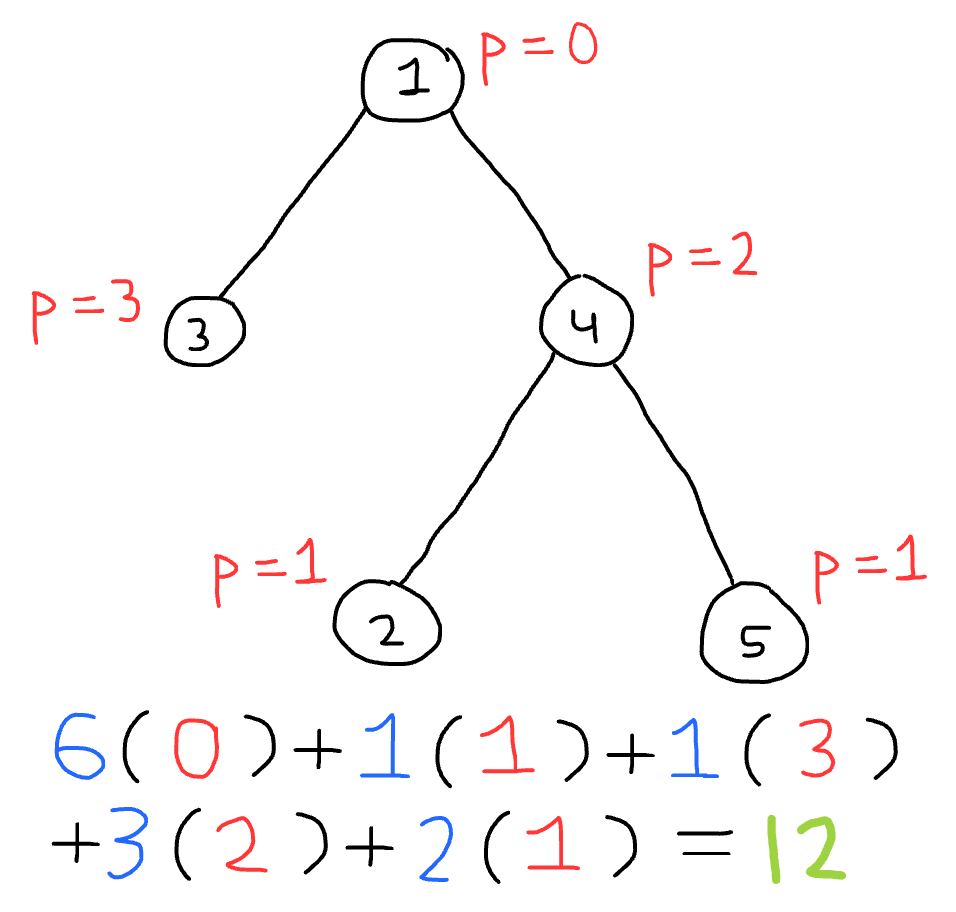
\includegraphics[scale=0.5]{Drawing-5.sketchpad.png}
\end{center}

The diagram above illustrates the first test case. An optimal set of operations to perform is to upgrade tower $3$ a total of $3$ times, upgrade tower $4$ twice, and upgrade towers $2$ and $5$ once each. This gives us a total cost of $12$, which is the minimum possible. Note that there may be other valid sets of operations with the same minimum cost.

\end{problem}

